\begin{figure}[h]
	\centering
	\missingfigure{Komponentendiagramm}		
	\caption{Komponentendiagramm - A}
	\label{fig:komponentendiagramm-a}
\end{figure}

\begin{tcolorbox}
Die strukturelle Übersicht des zu entwickelnden Systems wird mittels Komponentendiagrammen modelliert. 
Auf jedes Diagramm muss eine textuelle Beschreibung (Fließtext mit Umbrüchen / Absätzen oder Tabelle) folgen, in der die Aufgaben der Subkomponenten beschrieben werden. 
\end{tcolorbox}

\begin{figure}[h]
	\hspace{-3cm}
	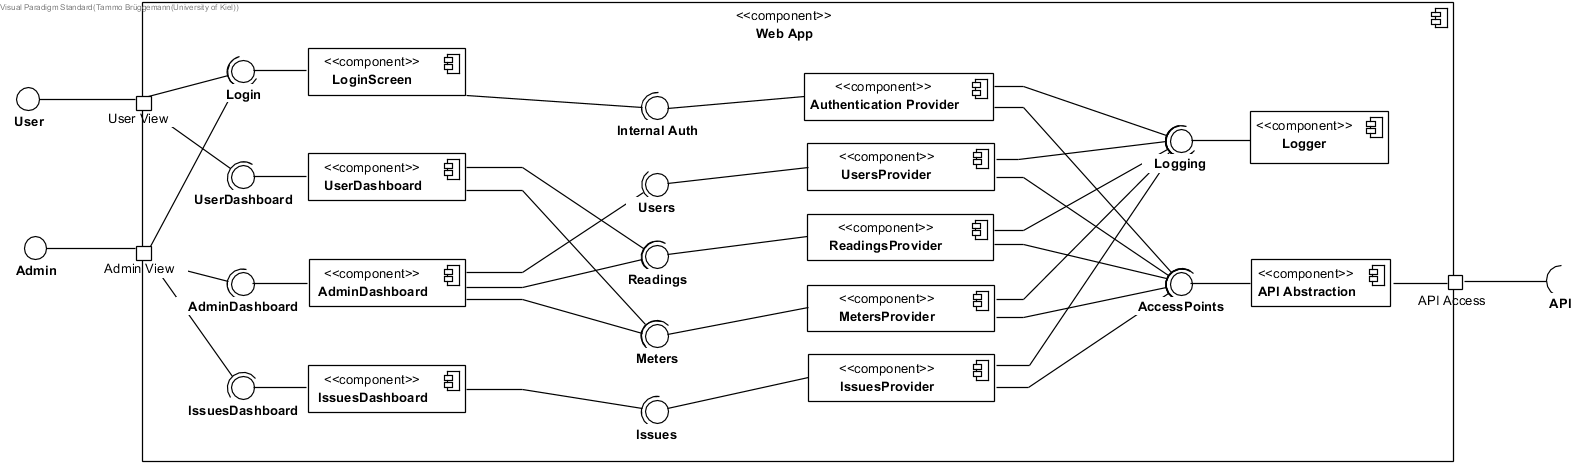
\includegraphics[scale = 0.73]{./img/Diagrams/Website-Components}
	Hier entsteht jetzt Text
\end{figure}
